\chapter{Application of remote sensing systems for assessment and prediction of different environmental risks}
\label{cha:literature}

	The remote sensing methods are reviewed in this chapter that are used to obtain indirect quantitative and qualitative properties about objects. Passive and active research methods are reviewed. The problems related to the large-scale processing of data for the operative retrieval of results about the object under study are reviewed. Methods for obtaining data from optical and radiometric satellite images are considered.

\section{Application of remote sensing data to the environment}
	Spatial data is one of the fastest growing scientific data, which poses significant computational difficulties for scientists who need to deal with the processing and analysis of large spatial data sets. With the continuous development of sensor technology, the volume of remote sensing images has increased rapidly in recent years and is expected to continue to do so (Yan Ma et al., 2015).
	
	Passive remote sensing data is often used for a variety of environmental challenges:
\begin{itemize}
	\item Wildfire prevention.
	\item Wildfire damage assessment.
	\item Optimization of nitrogen fertilization.
	\item Etc.
\end{itemize}

	For the prevention and detection of forest fire damage, a relative normalized deployment index can be applied (N. V. Rodinov), distinguishing cloud cover and hydrology from the total data array.

	The so-called change detection methodology (CD) can be used to determine forest fire damage. Using the CD methodology, images of different time sections of the same area are usually compared (N. V. Rodinov. Et al., 2016). In order to reduce the images present in the triggers (cloudiness, hydrology), filters are applied to distinguish such triggers using pixel algebra. In this case, the normalized deployment index is calculated for images of different time sections of the same area by making a relative estimate - a relative normalized deployment index. Based on the obtained research results, a data model distinguishing the places where the forest may be affected or most affected is presented.
	
	Currently, more than 100 spectral index variants used for different purposes have been described in different studies using passive remote sensing methods, but only a few of them find wide application in environmental research, monitoring (Vladimir Aleksandrovich Hamedov et al.). In many cases, the described indices do not provide an integrated approach to their complex use in observing a physical phenomenon, which is related to their applications in localized areas using empirical formulas in different ecosystems (Vladimir Aleksandrovis Hamedov et al.). It is for this reason that existing indices used to assess, for example, forest fire risk need to be adjusted for a specific area.
	
	In addition to passive remote sensing, active satellite surveys are increasingly being used, which, for example, make it possible to determine quite accurately:

\begin{itemize}
	\item Water surface contamination by oil products.
	\item Water surface contamination with plastic (plastic).
	\item Fire damage assessment.
	\item Improving fire risk indices.
	\item Etc.
\end{itemize}

	There are a lot of example of successful applying of remote sensing for monitoring and assessment various risk for different environmental purposes:

\begin{example} [Oil detection]
	\label{exa:oil}
	Petroleum products form a film on the surface of the water that is impermeable to sunlight. Without sunlight, the oxidation of bacteria and the multiplication and life of small organisms cease. The death of animal organisms damages the food web. The sea is often polluted by oil products during tanker accidents, but mainly due to sewage from tankers and refineries. Oil products pollute beaches, killing birds and fish.
	
	Large spills of oil products at sea can have significant biological and economic impacts.
	Public and media surveillance is usually intensive after a spill. Remote sensing is playing an increasingly important role in oil monitoring. Active satellite sensors SAR are commonly used to monitor marine oil spills. It is a more effective tool that can penetrate through clouds, rain and snow. The sensor emits microwave radiation that is reflected from the object and the received signal can be determined by the reversible scattering function (Merv Fing et al., 2014).
	
	Active satellite remote sensing has been successfully applied to simulate the 2010 oil spill in Dalian, Japan. In this study, a support vector machine was adapted to monitor oil spills based on high radiometric resolution SAR images (Jianchao Fana et al., 2015).
	
	Under different weather conditions in different places, the reflection and scattering properties of radio waves from the oil differ. On this basis, a vector machine can be constructed that can automatically classify oil spill zones (Jianchao Fana et al., 2015).
	In recent years, water has been increasingly contaminated with plastic products, which need to be monitored and identified to determine the extent of the contamination.
\end{example}

\begin{example}[Plastic detection]
	\label{exa:plastic}
	Plastic pollution in the ocean has been identified as a threat to various coastal areas. Many marine organisms can swallow or become entangled in plastic and this can pose a fatal risk to them. Although high concentrations of floating plastic debris are observed as they travel from inland waters to the open ocean, a detailed analysis of the spatial scale and abundance of waste is lacking and monitoring tools are not well developed to determine the distribution of pollution. Remote-sensing images with medium and high temporal, spectral, and spatial resolutions would be a great additional tool to quantify the distribution of floating marine plastic debris (Shungudzemwoyo P. Garabaa et al., 2017).
	
	Identifying plastics at sea is difficult because there are many different plastics in the marine environment. The size of the plastic can range from microplastics (less than 5 mm) to large plastic parts such as “ghost nets” (lost or discarded fishing nets). In the first case, the plastic material can be toxic through the absorption of contaminants into the plastic, and in the second case, the plastic contaminants can injure animals and endanger seafarers. Plastics can be made from granules used in manufacturing, from certain cosmetic and personal care products, from textile fibers (Lonneke Goddijn-Murphya et al., 2017).
	
	The rays of the sun falling on the surface of the water are partly reflected and the other partially penetrates through the surface. In water, light photons are absorbed and scattered in all directions. Due to the scattering and even distribution of repetitive light rays in all directions, it is possible to identify objects on the water surface. If the water is optically deep (the bottom is invisible), the fraction of light that is scattered and penetrates through the water into the air medium provides information on optically active (e.g., plankton) constituents of the water. Optically active components determine the apparent color of water, and their concentration can be calculated from spectral reflection measurements. In this case, the concentration of plastics can be identified in places where optically active water components cannot be identified (Lonneke Goddijn-Murphya et al., 2017).
	
	Satellites that have sensors that can detect the color of the ocean also provide instruments to identify the plastic, such as Sentinel-3 working in conjunction with Sentinel-3 SLSTR comparing nine bands VIS-SWIR 0.55–12 {$\mu$}m (Lonneke Goddijn-Murphya et al., 2017).
\end{example}

\begin{example} [Nitrogen of plants detection ]
	\label{exa:nitro}
	Optical satellite imagery is by far the most suitable for determining the nitrogen content of plants to reduce the use of fertilizers in crop production.
\end{example}

\begin{example} [Title]
	Write more about how remote sensing is used for fire assessment ant prediction
\end{example}

\section{ESO (European Space Agency) is developing a Sentinel satellite system under the Copernicus program}

	There is an increasing need for operative analysis in the territory in question to solve various environmental, landscaping and risk management tasks. Such an analysis requires access to constantly updated and high-resolution remote sensing data. Such data are provided by ESO (European Space Agency) under the Copernicus program. The paper examines the application of open Sentinel-1 and Sentinel-2 satellite remote sensing data to address a risk management task, such as fire damage detection.
	
	Sentinel remote sensing data are being developed by ESA under the Copernicus program. This data is free and freely available. In recent years, the need for access to open, free, and frequently updated time-lapse remote sensing data has been growing. Sentinel is divided into 6 groups of satellites, each of which has 2 satellites that can be used to solve various environmental, landscaping and risk management tasks.
	
	One of the most common tasks is risk management. Sentinel data, due to their accuracy and frequent updating in the time section, can be used, for example, to determine fire damage.
	
	ESA has launched two satellites from each Sentinel family into orbit under the ongoing Copernicus program:
	
\begin{itemize}
	\item Sentinel-1 - satellites using active remote sensing sensors. Sentinel-1A launched into orbit in 2014 and Sentinel-1B in 2016.
	\item Sentinel-2 - satellites using multi-spectral high-resolution passive remote sensing sensors. Sentinel-2A was launched into orbit in 2015, and Sentinel-2B in 2017.
	\item Sentinel-3 - multi-functional satellites are used for seabed topography, sea and land surface temperature determination. Used to monitor the environment and climate change. Sentinel-3A was released in 2016 and Sentinel-3B was released in 2018.
	\item Sentinel-4 - geostationary orbit satellites for atmospheric observation.
	\item Sentinel-5 - polar orbit satellites for atmospheric monitoring.
	\item Sentinel-6 is a satellite using an altimeter radar that measures the world's sea level. Used for oceanography and climate research.
\end{itemize}

	Sentinel satellite data is free and publicly available. To receive them, it is necessary to register on the Copernicus Hub website and download them according to the selected search criteria (time, place, etc.). Figure \ref{fig:copernicus_hub} shows a graphical user interface that can be used to download data.

\begin{figure}[H]
	\centering
	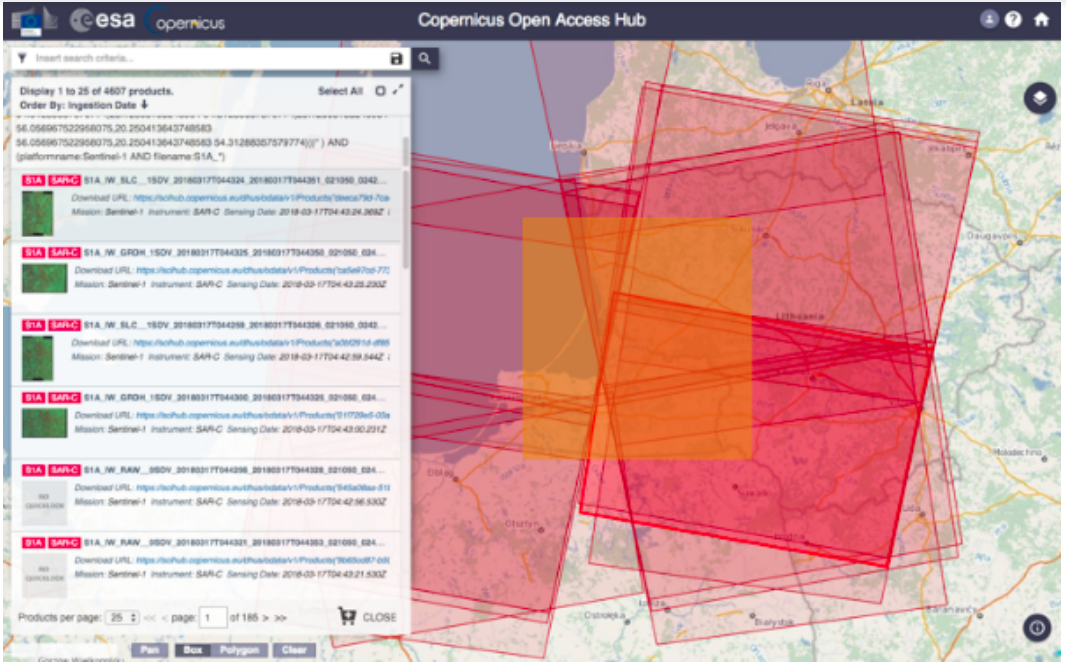
\includegraphics[width=0.8\linewidth]{images/copernicus_hub.png}
	\caption{Sentinel data download via the Copernicus Hub website}
	\label{fig:copernicus_hub}
\end{figure}

	Also the Copernicus Hub programming interface can be used to automate data downloads by specified parameters.
	
	Sentinel data is provided in SAFE (Standard Archive Format for Europe) format. This format stores not only raster information but also textual information that can be used to correct raster data.

\begin{figure}[H]
	\centering
	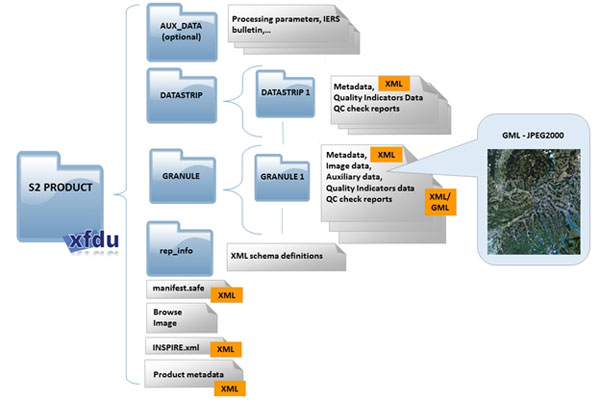
\includegraphics[width=0.8\linewidth]{images/sentinel-2_data_formats.jpg}
	\caption{Example of Sentinel-2 data format}
	\label{fig:sentinel-2_format}
\end{figure}

	The Copernicus program, developed by ESA, provides high-quality and freely available Sentinel satellite data that can be adapted to meet a variety of GIS challenges. One example of such tasks is the identification of fire damage to the forest, the detection of oil spills at sea, the identification of plastic sites at sea. ESA provides all the tools needed for data retrieval (Coperinicus Hub data download portal) and GIS analysis (SNAP software). Sentinel data is high quality, frequently updated, and SNAP free software provides all the tools to perform GIS analysis for both scientific and commercial purposes.

\section{Sentinel passive and active remote sensing systems}
	Remote sensing is the process of obtaining qualitative and quantitative data about a particular object without physical contact.
	Remote sensing systems can be divided into passive and active systems using electromagnetic radiation:
	
	\begin{itemize}
		\item Passive remote sensing systems use an external source of electromagnetic radiation, usually the sun.
		\item Active remote sensing systems have their own light source, which is an electromagnetic wave generator that emits waves from a satellite to the earth's surface. The reflected waves from the earth's surface are captured by a satellite.
	\end{itemize}

	ESA has launched two satellites from each Sentinel family into orbit under the ongoing Copernicus program:
	
	\begin{itemize}
		\item Sentinel-1 - satellites using active remote sensing sensors. Sentinel-1A launched into orbit in 2014 and Sentinel-1B in 2016.
		\item Sentinel-2 - satellites using multi-spectral high-resolution passive remote sensing sensors. Seintinel-2A was launched into orbit in 2015, and Sentinel-2B in 2017.
	\end{itemize}

	Sentinel data is presented in SAFE (Standard Archive Format for Europe) format, which stores not only raster information but also text that can be used to correct raster data, such as cloud cover, so ESA recommends the use of SNAP (Figure 4) open source software for the processing and analysis of their data (\url{http://www.eo4sd-eastern.eu/sites/default/files/publications/snap_workbook_english.pdf}).
	
	Since 2014, radar data (SAR) from the European satellite Sentinel-1A have been freely available, opening up new opportunities for research. The Copernicus portal provides many examples of where they can be applied, ranging from the detection of forest fire damage to the detection of oil spills in water bodies. The main parameters, for example, of Sentinel-1A radar photos (E.A. Baldina et al., 2016):
	
	{\setlength{\extrarowheight}{15pt}%
	\begin{table}[H]
		\begin{center}
			\caption{Sentinel-1A satellite data parameters (E.A. Baldina et al., 2016)}
			\label{tab:sent-char}
			\begin{tabularx}{\textwidth}{|X|X|X|X|}
				\hline
				\textbf{Mode} & \textbf{Coverage area, km} & \textbf{Spatial resolution, m} & \textbf{Polarization\newline(H - horizontal;\newline V - vertical)}\\
				\hline
				Stripmap (SM) & 80 & 5x5 & HH, VV, HH+VV, VV+VH \\
				\hline
				Interferometric Wide Swath (IW) & 250 & 5x20 & HHH, VV, HH+HV, VV+VH \\
				\hline
				Extra-Wide Swath (EW) & 400 & 20x40 & HH, VV, HH+HV, VV+VH \\
				\hline
				Wave (WV) & 20x20 & 5x5 & HH, VV \\
				\hline
			\end{tabularx}
		\end{center}
	\end{table}

	The resolution of the data received by the Sentinel-2A satellite depends on the color wave captured by the sensor and ranges from 10 m to 60 m (\ref{tab:sent-res})).
	
	{\setlength{\extrarowheight}{15pt}%
	\begin{table}[H]
		\begin{center}
			\caption{Sentinel-2A satellite data resolution (Du, Y et al., 2016)}
			\label{tab:sent-res}
			\begin{tabularx}{\textwidth}{|X|X|X|}
				\hline
				\textbf{Physical band} & \textbf{Pixel resolution, m} & \textbf{Wave length, mm}\\
				\hline
				B1 & 60 & 443 \\
				\hline
				B2 & 10 & 490 \\
				\hline
				B3 & 10 & 560 \\
				\hline
				B4 & 10 & 665 \\
				\hline
				B5 & 20 & 705 \\
				\hline
				B6 & 20 & 740 \\
				\hline
				B7 & 20 & 783 \\
				\hline
				B8 & 10 & 842 \\
				\hline
				B8A & 20 & 865 \\
				\hline
				B9 & 60 & 945 \\
				\hline
				B10 & 60 & 1375 \\
				\hline
				B11 & 20 & 1610 \\
				\hline
				B12 & 20 & 2190 \\
				\hline
			\end{tabularx}
		\end{center}
	\end{table}
		
	